\documentclass[9pt, aspectratio=169]{beamer}
\usepackage{FiraSans}
\usetheme[subsectionpage=progressbar]{metropolis}
\usepackage[utf8]{inputenc}
\usepackage{amsmath}
\usepackage{amsfonts}
\usepackage{amssymb}
\usepackage{multicol}
\usepackage{tikz}
\usetikzlibrary{matrix}
\usepackage{caption}
\usepackage{xcolor}
\usepackage[T1]{fontenc} 
\usepackage[skins]{tcolorbox}
\author{Nicola Roman\`o - nicola.romano@ed.ac.uk}
\title{Lecture 13 - CNN architectures}
\setlength{\fboxsep}{0pt}
\setbeamertemplate {footline}{\begin{scriptsize}\hfill\insertframenumber ~of \inserttotalframenumber\kern1em\vskip5pt\end{scriptsize}}

% Remove "Figure" in front of captions
% See https://tex.stackexchange.com/questions/82456/how-to-remove-figure-caption-prefix-figure-in-beamer
\captionsetup{labelformat=empty,labelsep=none}

\titlegraphic{\centering \includegraphics[scale=.5]{instituteLogo.png}}
\date{}

\begin{document}

\newtcolorbox{codebox}{enhanced,
    top=2pt,
    left=2pt,
    right=2pt,
    bottom=2pt,
    boxrule=0pt,
    leftrule=5pt,
    sharp corners,
    colback=gray!20,
    colframe=blue!60!black}

\begin{frame}
    \titlepage
\end{frame}

\begin{frame}
    {Introduction}

    Today we are going to discuss a few classic papers using CNN for image analysis.

    We will analyse the following architectures:

    \begin{itemize}
        \item LeNET-5
        \item AlexNet
        \item VGG
        \item GoogLeNet
        \item ResNet
    \end{itemize}

    The idea is to get some \textbf{intuition} about these architectures and how they work.
\end{frame}

\begin{frame}
    {Learning objectives}
    \begin{columns}
        \begin{column}{0.8\textwidth}
            \begin{itemize}
                \item Describe commonly used patterns in CNN architectures
                \item Describe and explain the advantages of different CNN architectures
            \end{itemize}
        \end{column}
        \begin{column}{0.2\textwidth}
            
\includegraphics[angle=-30, origin=tr, width=1.5\textwidth]{lightbulb.png}
        \end{column}
    \end{columns}
\end{frame}

\section{LeNET-5}

\begin{frame}
    {LeNET-5}
    \begin{itemize}
        \item "Gradient Based Learning Applied to Document Recognition", Yann LeCun et al. 1998
        \item A seminal paper describing the use of CNN in image analysis
        \item Simple architecture with convolutional layers, average pooling and fully-connected layers
        \item Task: recognition of handwritten digits to be used for processing of bank cheques
    \end{itemize}
\end{frame}

\begin{frame}
    {LeNet-5 architecture}
    \centering
    \includegraphics[width=\textwidth]{LeNet-5.png}
\end{frame}

\begin{frame}
    {LeNet-5 training}

    \begin{itemize}
        \item Trained on MNIST dataset (60000 handwritten digits)
        \item Error rate: <1\%
    \end{itemize}

    \centering
    \includegraphics[width=.4\textwidth]{lenet5_training.png}
    \includegraphics[width=.4\textwidth]{lenet5_missclassification.png}
\end{frame}

\begin{frame}
    {LeNet-5 take home points}
    \begin{itemize}
        \item A simple architecture with convolutional layers, average pooling and fully-connected layers
        \item Introduced the $[\text{Conv}+\text{Pool}]_n + FC$ pattern
        \item This is mostly interesting from a historical perspective, not really used nowadays.
    \end{itemize}
\end{frame}

\section{AlexNet}
\begin{frame}
    {AlexNet}
    \begin{itemize}
        \item "ImageNet Classification with Deep Convolutional
              Neural Networks", Alex Krizhevsky et al. 2012
        \item Widely considered as one of the most influential papers that boosted research in CNN for image analysis
        \item Similar architecture to LeNet-5, but with more convolutional layers
        \item Much bigger network (LeNet-5 ~60k parameters, AlexNet ~60M parameters)
        \item Winner of the ImageNet Large Scale Visual Recognition Challenge (ILSVRC) in 2012.
    \end{itemize}
\end{frame}

\begin{frame}
    {The ImageNet Large Scale Visual Recognition Challenge}
    \begin{columns}
        \begin{column}{.5\textwidth}
            \begin{itemize}
                \item \href{https://www.image-net.org}{\underline{ImageNet}} is a database of images of various objects, used for training and testing deep neural networks.
                \item Introduced in Deng et al., 2009 - ImageNet: A large-scale hierarchical image database
                \item It contains >14 million images of various objects, labelled with >20000 classes.
                \item The ILSVRC is a competition to define new algorithms for image classification.
                \item ILSVRC uses a subset of ImageNet, containing 1000 classes and ~1.3M training images, 50k validation images and 100k test images.
            \end{itemize}
        \end{column}
        \begin{column}{.5\textwidth}
            \includegraphics[width=\textwidth]{imagenet.png}
        \end{column}
    \end{columns}
\end{frame}

\begin{frame}
    {AlexNet architecture}
    \centering
    \includegraphics[width=\textwidth]{AlexNet.png}
\end{frame}

\begin{frame}
    {Improvements in AlexNet}
    AlexNet introduced a number of improvements:

    \begin {itemize}
    \item ReLU activation function (instead of sigmoid/tanh)
    \item Dropout
    \item Softmax activation function in the last layer
    \item Data augmentation
    \item \color{gray}Local response normalization
    \item Training on multiple GPUs
    \end {itemize}
\end{frame}

\begin{frame}
    {ReLU activation function}
    \centering
    \includegraphics[width=\textwidth]{alexnet_relu.png}

    Introduction of the ReLU activation function (instead of sigmoid/tanh) allowed to train much faster.
\end{frame}

\begin{frame}
    {Dropout}
    \begin{itemize}
        \item A type of "regularization" technique, used to prevent overfitting
        \item A random subset of the weights is set to zero at each training step.
        \item Originally introduced in "Dropout: A Simple Way to Prevent Neural Networks from Overfitting", Srivastava et al. 2014
    \end{itemize}

    \centering
    \only<1>{
        \includegraphics[width=\textwidth]{dropout.png}
    }
    \only<2>{
        \includegraphics[width=.5\textwidth]{dropout_error.png}
    }

    \footnotesize
    \raggedright
    Srivastava et al. 2014
\end{frame}

\begin{frame}
    {The softmax activation function}
    \begin{itemize}[<+->]
        \item Generalization of the logistic function to multiple classes
        \item Common choice for classification problems in ANNs.
        \item Defined as \Large $$S(y_i) = \frac{{e}^{y_i}}{\sum_j{e^{y_j}}}$$
        \item \normalsize It is used in the last layer of a CNN to compute the probability of each class.
    \end{itemize}

    \only<5>{
        \centering
        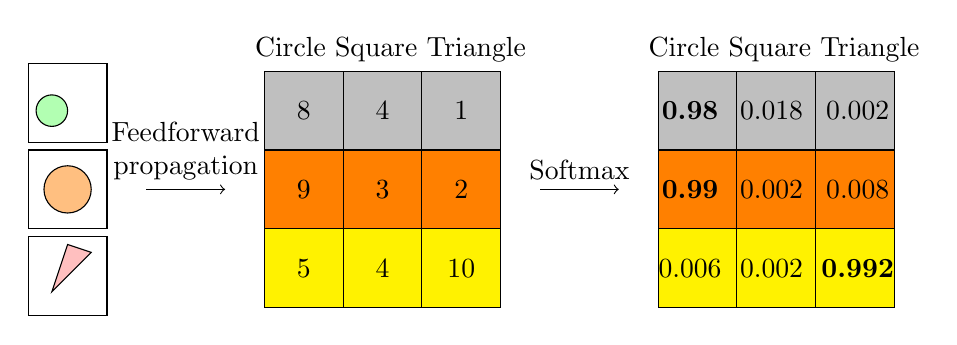
\begin{tikzpicture}
            \foreach \y in {-0.1, 1, 2.1}
                {
                    \draw [fill=white] (0, \y) rectangle (1, \y + 1);

                }

            \foreach \x in {3, 4, 5, 8, 9, 10}
                {
                    \draw [fill = yellow] (\x, 0) rectangle (\x + 1, 1);
                    \draw [fill = orange] (\x, 1) rectangle (\x + 1, 2);
                    \draw [fill = gray!50!white] (\x, 2) rectangle (\x + 1, 3);
                }

            \draw [fill=pink] (0.3, 0.2) -- (0.8, 0.7) -- (0.5, 0.8) -- cycle;
            \draw [fill=orange!50!white] (0.5, 1.5) circle (0.3);
            \draw [fill=green!30!white] (0.3, 2.5) circle (0.2);

            \node [align=center, anchor=south] at (4.6, 3) {Circle~Square~Triangle};
            \node [align=center, anchor=south] at (9.6, 3) {Circle~Square~Triangle};

            \matrix (m) [matrix of nodes, ampersand replacement=\&, nodes={anchor=center, minimum width=1cm, minimum height = 1cm}] at (4.5, 1.5)
            {
                8 \& 4 \& 1  \\
                9 \& 3 \& 2  \\
                5 \& 4 \& 10 \\
            };

            \matrix (m) [matrix of nodes, ampersand replacement=\&, nodes={anchor=center, minimum width=1cm, minimum height = 1cm}] at (9.5, 1.5)
            {
                \textbf{0.98} \& 0.018 \& 0.002 \\
                \textbf{0.99} \& 0.002 \& 0.008 \\
                0.006 \& 0.002 \& \textbf{0.992} \\
            };

            \draw [->] (1.5, 1.5) -- (2.5, 1.5) node [above, midway, text width=8em, align=center, anchor = south] {Feedforward propagation};
            \draw [->] (6.5, 1.5) -- (7.5, 1.5) node [above, midway] {Softmax};
        \end{tikzpicture}
    }
\end{frame}

\begin{frame}
    {AlexNet take home points}
    \begin{itemize}
        \item Similar architecture to LeNet-5, but with more convolutional layers
        \item \textbf{ReLU activation functions} - faster computation, more efficient training
        \item \textbf{Dropout} to prevent overfitting
        \item Training on multiple GPUs
    \end{itemize}
\end{frame}

\section{VGG}

\begin{frame}
    {VGG}
    \begin{itemize}
        \item "Very Deep Convolutional Networks for Large-Scale Image Recognition", Karen Simonyan and Andrew Zisserman, 2015
        \item Very popular architecture for image analysis
        \item Very deep network, with 16 layers (VGG-16) or 19 layers (VGG-19). ~130M parameters
        \item Winner of ILSVRC in 2015.
        \item VGG-19 is slightly better, but more computationally expensive (in practice VGG-16 more common).
    \end{itemize}
\end{frame}

\begin{frame}
    {VGG architecture}
    \centering
    \includegraphics[width=.7\textwidth]{VGG16.jpg}
\end{frame}

\begin{frame}
    {VGG take home points}
    \begin{itemize}
        \item Very deep network, ~130M parameters
        \item Uses small convolutions (3x3) with stride 1
        \item All layers have same configuration (simplified hyperparameter choice)
        \item $1\times 1$ convolutions to increase non-linearity
    \end{itemize}
\end{frame}
\section{GoogLeNet}
\begin{frame}
    {GoogLeNet}
    \begin{columns}
        \begin{column}{.5\textwidth}
            \begin{itemize}
                \item "Going Deeper with Convolutions", Szegedy et al. 2014
                \item Moves away from the structure we've seen so far
                \item Introduces "Inception" modules
                \item 12x less parameters than AlexNet but much more accurate!
                \item Newer versions (Inception v3, v4) have more powerful architectures
            \end{itemize}
        \end{column}
        \begin{column}{.5\textwidth}
            \centering
            \includegraphics[width=\textwidth]{WeNeedToGoDeeper.jpg}
        \end{column}
    \end{columns}
\end{frame}

\begin{frame}
    {GoogLeNet architecture}
    \centering
    \includegraphics[width=\textwidth]{GoogLeNet.png}
\end{frame}

\begin{frame}
    {Inception module}
    \begin{itemize}
        \item The inception module is a building block of the GoogLeNet architecture
        \item It is a combination of convolutions with different kernel sizes
        \item It is a way to increase the non-linearity of the network
        \item It is a way to reduce the number of parameters
    \end{itemize}

    \centering
    \includegraphics[width=.4\textwidth]{inception_naive.png}
    \pause
    \includegraphics[width=.4\textwidth]{inception_dimred.png}

\end{frame}

\begin{frame}
    {GoogLeNet take home points}
    \begin{itemize}
        \item 22 layers
        \item Heavily relies on $1\times 1$ convolutions
        \item Inception modules allow multi-scale feature extraction
        \item Drops FC layers
        \item Extra "side" classifications to improve gradient optimization in earlier layers
    \end{itemize}
\end{frame}

\section{ResNet}

\begin{frame}
    {ResNet}
    \begin{itemize}
        \item He 2015 - Deep Residual Learning for Image Recognition
        \item Tackles the problem of degraded performance in larger networks
        \item Introduces \textit{skip connections} between layers
        \item Up to 1000+ layers!
    \end{itemize}
\end{frame}

\begin{frame}
    {ResNet architecture}
    \centering
    \includegraphics[width=\textwidth]{resnet.png}
\end{frame}

\begin{frame}
    {The problem with deep networks}
    As we add more layers, the network becomes more difficult to train

    \centering
    \includegraphics[width=.7\textwidth]{resnet_big_small_network.png}

    This is surprising because we expect a deeper network to be at least as good as a shallower network. Indeed the extra layers could "simply" learn the identity function $I(x) = x$.
\end{frame}

\begin{frame}
{Skip connections}
By adding a skip connection, the network can learn the residual function $F(x) = H(x) - x$. The intuition is that the residual function is easier to learn than the identity function as you could simply zero out some of the layers.

\centering
\includegraphics[width=.4\textwidth]{resnet_identity.png}
\end{frame}

\begin{frame}
{Skip connections improve performance}
\centering
\includegraphics[width=\textwidth]{resnet_training.png}
\end{frame}

\begin{frame}
    {ResNet take home points}
    \begin{itemize}
        \item Very deep network (up to 1000+ layers)
        \item Uses \textit{skip connections} between layers
        \item Uses \textit{bottleneck} blocks (similar to GoogLeNet)
    \end{itemize}
\end{frame}

\begin{frame}
    {Comparison of CNN architectures}
    \centering
    \includegraphics[width=\textwidth]{comparison.png}
\end{frame}

\begin{frame}
    {Transfer learning}
    \only <1>{
        \begin{itemize}
            \item Training a CNN is expensive in terms of time and computer memory.
            \item Luckily, you can make use of pre-trained models to speed up the training process!
            \item This process is called \textbf{transfer learning}.
            \item For example, if you wanted to classify images, rather than start from scratch you could begin with VGG-16, or with GoogLeNet and modify them for your needs! (i.e. do not reinvent the wheel!)
        \end{itemize}
    }
    \centering
    \begin{tikzpicture}[scale=0.9]
        \only <2->{
            % Generic images
            \node[inner sep=0pt] (generic) at (0,2)
            {\includegraphics[height=2.5cm]{genericimages.png}};
            \node (label) at (0, 0) {Generic images};

            % Top CNN
            % Conv layers
            \foreach \x [count=\N] in {2.5,3,...,5}
                {
                    \node (layer\N) [draw, rectangle, fill=orange!50!yellow, minimum width=1, minimum height=3cm-0.4*\N cm] at (\x,1.5) {};
                }
            % FC layers
            \foreach \x [count=\N from 7] in {6,6.5,7}
                {
                    \node (layer\N) [draw, rectangle, fill=blue!50!yellow, minimum width=1, minimum height=2.5cm-.1*\N cm] at (\x,1.5) {};
                }
            \node [text width=4em] (layer10) at (9.5, 1.5) {Dog, Cat, Plane, \dots};
            % Arrows
            \foreach \N [count=\Nn from 2] in {1,2,...,9}
                {
                    \draw [->] (layer\N) -- (layer\Nn.west);
                }
            \node [right of=label, node distance=6cm] {\textit{"Template"} CNN - e.g. VGG-16};

            \only<3>{
                % Domain specific images
                \node[inner sep=0pt] (generic) at (0,-2)
                {\includegraphics[height=2.5cm]{bioimages.png}};
                \node at (0, -4) {Task-specific images};

                % Bottom CNN
                % Conv layers
                \foreach \x [count=\N] in {2.5,3,...,4.5}
                    {
                        \node (layer_bottom_\N) [draw, rectangle, fill=orange!50!yellow, minimum width=1, minimum height=3cm-0.4*\N cm] at (\x,-2) {};
                    }
                \node (layer_bottom_6) [draw, rectangle, fill=green!40!yellow, minimum width=1, minimum height=0.6cm] at (5,-2) {};

                % FC layers
                \foreach \x [count=\N from 7] in {6,6.5,7}
                    {
                        \node (layer_bottom_\N) [draw, rectangle, fill=green!60!yellow, minimum width=1, minimum height=2.5cm-.1*\N cm] at (\x,-2) {};
                    }

                \node [text width=4em] (layer_bottom_10) at (9.5, -2) {Liver, Kidney, Bone, Retina, \dots};
                \node [color=orange!80!black] at (4, 4) {\textbf{Conv layers}};
                \node [color=blue!50!yellow] at (6.5, 4) {\textbf{FC layers}};
                \draw [color=orange, line width=1pt] (2.2,-3.7) -- (4.8,-3.7) node [below, midway] {Keep};
                \draw [color=green!50!black, line width=1pt] (5,-3.7) -- (8,-3.7) node [below, midway] {Retrain};
                % Arrows
                \foreach \N [count=\Nn from 2] in {1,2,...,9}
                    {
                        \draw [->] (layer_bottom_\N) -- (layer_bottom_\Nn.west);
                    }
            }
        }
    \end{tikzpicture}
\end{frame}

\end{document}

